\subsection{Z 变换}

Z 变换是离散时间信号与系统的理论研究中的一种重要的数学工具。
它把离散的数学模型(差分方程)转换为简单的代数方程,
使其求解过程得以简化。

\subsubsection{Z 变换的定义}

\begin{definition}[Z 变换的定义]
    设 $x(n)$ 是一个离散时间信号,其\bd{单边 Z 变换}的定义为
    \begin{align*}
        X(z) = \sum_{n = 0}^{+\infty} x(n) z^{-n},
    \end{align*}
    \bd{双边 Z 变换}的定义为
    \begin{align*}
        X(z) = \sum_{n=-\infty}^{+\infty} x(n) z^{-n},
    \end{align*}
    记作 $X(z) = \mathcal{Z}[x(n)]$。
\end{definition}

\begin{remark}[Z 变换和 DTFT 之间的关系]
    回忆 DTFT 的定义,我们有
    \begin{align*}
        X(\omega) = \sum_{n=-\infty}^{+\infty} x(n) \mathe^{-\mathi\omega n},
    \end{align*}
    注意到 $\mathe^{-\mathi\omega n} = \left(\mathe^{\mathi\omega}\right)^{-n}$,
    因此,DTFT 也可以写为
    \begin{align*}
        X(\omega) = \sum_{n=-\infty}^{+\infty} x(n) \left(\mathe^{\mathi\omega}\right)^{-n},
    \end{align*}
    这具有类似于 Z 变换的形式。DTFT 的变换核是 $\mathe^{-\mathi\omega n}$,
    将其换成 $z^{-n}$,可以看做是变换核对应的取值从单位圆上的点($\mathe^{\mathi\omega}$)
    变成了整个复平面上的点($z$)。
\end{remark}

\subsubsection{Z 变换的收敛域}

\begin{definition}[Z 变换的收敛域]
    考虑 Z 变换
    \begin{align*}
        X(z) = \mathcal{Z}[x(n)] = \sum_{n=-\infty}^{+\infty} x(n) z^{-n},
    \end{align*}
    它具有幂级数求和的形式。显然当 $z$ 固定时,它不一定对所有的序列 $x(n)$ 都收敛;
    当序列 $x(n)$ 固定时,它不一定对所有的 $z$ 都收敛。

    但如果给定了序列 $x(n)$,则可以求出使得 $X(z)$ 收敛的 $z$ 的取值范围。
    我们称使 $X(z)$ 收敛的 $z$ 的取值范围为 $X(z)$ 的\bd{收敛域},简记为 ROC。
\end{definition}

\begin{property}[Z 变换的 ROC 的性质]
    Z 变换的 ROC 一般具有以下性质:
    \begin{enumerate}
        \item ROC 的一般形式是复平面上以原点为中心的圆环。
        \item ROC \bd{不包含极点},而且常以极点作为 ROC 的边界。
        \item 在 ROC 内,ZT 及其导数是 $z$ 的连续函数,即 ZT 是 ROC 内每一点的解析函数。
    \end{enumerate}
\end{property}

\begin{example}[Z 变换 ROC 的求解]
    Z 变换得到的序列是一个幂级数,幂级数的收敛域称为\bd{收敛圆},
    收敛圆的半径称为幂级数的\bd{收敛半径}。收敛半径的求法有两种:
    \begin{itemize}
        \item 利用比值判别法,
            \begin{align*}
                \lim_{n \to +\infty}\abs{\frac{a_{n+1}}{a_n}} = \rho.
            \end{align*}
        \item 利用根值判别法,
            \begin{align*}
                \lim_{n \to +\infty}\sqrt[n]{\abs{a_n}} = \rho.
            \end{align*}
    \end{itemize}
    收敛半径 $R$ 与 $\rho$ 的关系为:
    \begin{itemize}
        \item 若 $\rho = 0$,则 $R = +\infty$。
        \item 若 $\rho = +\infty$,则 $R = 0$。
        \item 对于其他情况,$R = 1/\rho$。
    \end{itemize}
\end{example}

\begin{property}[有限长序列的 ROC]
    \bd{有限长序列} $x(n)$ 在 $n < n_1$ 或 $n > n_2$ 时为 $0$,
    则其 Z 变换为
    \begin{align*}
        X(z) = \sum_{n=n_1}^{n_2} x(n) z^{-n},
    \end{align*}
    其中 $n_1 < n_2$。其 ROC \bd{至少}是 $0 < \abs{z} < +\infty$。

    序列的左右端点只会影响其在 $z = 0$ 和 $z = +\infty$ 处的收敛性:
    \begin{itemize}
        \item 若 $n_1 < 0 < n_2$,则 ROC 为 $0 < \abs{z} < +\infty$。
        \item 若 $n_1 < n_2 \le 0$,则 ROC 为 $0 \le \abs{z} < +\infty$。
        \item 若 $0 \le n_1 < n_2$,则 ROC 为 $0 < \abs{z} \le +\infty$。
    \end{itemize}
\end{property}

\begin{property}[右边序列的 ROC]
    \bd{右边序列} $x(n)$ 在 $n < n_1$ 时为 $0$,则其 Z 变换为
    \begin{align*}
        X(z) = \sum_{n=n_1}^{+\infty} x(n) z^{-n}.
    \end{align*}
    若满足
    \begin{align*}
        \lim_{n \to +\infty}\sqrt[n]{\abs{x(n)z^{-n}}} < 1,
    \end{align*}
    则右边序列的收敛域为
    \begin{align*}
        \abs{z} > \lim_{n \to +\infty}\sqrt[n]{\abs{x(n)}} = R_{x1}.
    \end{align*}
    因此,\bd{右边序列的 ROC 是半径为 $R_{x1}$ 的圆外部分}。

    序列的左右端点只会影响其在 $z = +\infty$ 处的收敛性:
    \begin{itemize}
        \item 若 $n_1 < 0$,则 ROC 为 $R_{x1} < \abs{z} < +\infty$。
        \item 若 $n_1 \ge 0$,则 ROC 为 $R_{x1} < \abs{z} \le +\infty$。
    \end{itemize}
\end{property}

\begin{property}[左边序列的 ROC]
    \bd{左边序列} $x(n)$ 在 $n > n_2$ 时为 $0$,则其 Z 变换为
    \begin{align*}
        X(z) = \sum_{n=-\infty}^{n_2} x(n) z^{-n}.
    \end{align*}
    若满足
    \begin{align*}
        \lim_{n \to +\infty}\sqrt[n]{\abs{x(-n)z^n}} < 1,
    \end{align*}
    则左边序列的收敛域为
    \begin{align*}
        \abs{z} < \frac{1}{\lim_{n \to +\infty}\sqrt[n]{\abs{x(-n)}}} = R_{x2}.
    \end{align*}
    因此,\bd{左边序列的 ROC 是半径为 $R_{x2}$ 的圆内部分}。

    序列的左右端点只会影响其在 $z = 0$ 处的收敛性:
    \begin{itemize}
        \item 若 $n_2 > 0$,则 ROC 为 $0 < \abs{z} < R_{x2}$。
        \item 若 $n_2 \le 0$,则 ROC 为 $0 \le \abs{z} < R_{x2}$。
    \end{itemize}
\end{property}

\begin{property}[双边序列的 ROC]
    \bd{双边序列}在所有 $n$ 处均有定义,可以将其看成左边序列和右边序列的组合。
    \begin{align*}
        X(z) = \sum_{n=-\infty}^{+\infty} x(n) z^{-n} = \sum_{n=0}^{+\infty} x(n) z^{-n} + \sum_{n=-\infty}^{-1} x(n) z^{-n}.
    \end{align*}
    则有
    \begin{align*}
        R_{x1} = \lim_{n \to +\infty}\sqrt[n]{\abs{x(n)}}, \quad R_{x2} = \frac{1}{\lim_{n \to +\infty}\sqrt[n]{\abs{x(-n)}}}.
    \end{align*}
    若 $R_{x1}$ 和 $R_{x2}$ 均存在,且 $R_{x1} < R_{x2}$,则双边序列的 ROC 为
    \begin{align*}
        R_{x1} < \abs{z} < R_{x2}.
    \end{align*}
    否则,ROC 为空集,即,双边序列的 Z 变换不存在。
\end{property}

\begin{remark}[ROC 与极点的关系]
    序列的 ROC 以极点为边界,是连通的区域,且内部不包含极点。
    \begin{figure}[H]
        \centering
        \begin{tabular}{|c||c|}
            \hline
            右边序列 & 以其模最大的有限极点的模为半径的圆外面的区域(不包括圆周) \\
            \hline
            左边序列 & 以其模最小的非零极点的模为半径的圆内部的区域(不包括圆周) \\
            \hline
            双边序列 & 以模的大小相邻的两个极点的模为半径的两个圆所形成的圆环区域(不包括两圆周) \\
            \hline
        \end{tabular}
    \end{figure}
    如图 \ref{fig:roc_pole} 所示,灰色区域为 ROC,蓝色虚线为 ROC 边界,红色实线为 $\abs{z} = 1$ 的单位圆,
    绿色叉号为极点。左上角的图片是右边序列,左下角的图片是左边序列,右边的图片是双边序列。
    \begin{figure}[H]
        \centering
        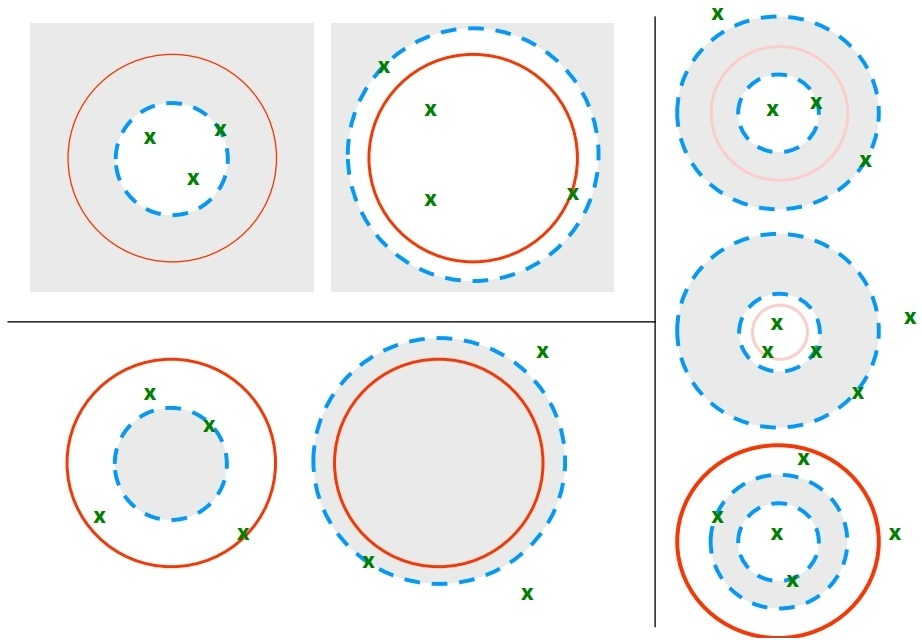
\includegraphics[width=0.6\textwidth]{chap4/img/roc_pole.png}
        \caption{ROC 与极点的关系}
        \label{fig:roc_pole}
    \end{figure}
\end{remark}

\begin{note}
    求 ROC 所求得的是级数收敛的\bd{充分条件而非必要条件},
    即,实际上 ROC 可能比所求得的更大。
\end{note}

\subsubsection{常见序列及其 ZT}

\begin{example}[单位冲激序列的 ZT]
    单位冲击序列 $\delta(n)$ 的 Z 变换为
    \begin{align*}
        \mathcal{Z}[\delta(n)] = 1, \quad (\text{ROC}: 0 \le \abs{z} \le +\infty).
    \end{align*}
    这是因为
    \begin{align*}
        \mathcal{Z}[\delta(n)] = \sum_{n=-\infty}^{+\infty} \delta(n) z^{-n} = \delta(0) = 1.
    \end{align*}
\end{example}

\begin{example}[单位阶跃序列的 ZT]
    单位阶跃序列 $u(n)$ 的 Z 变换为
    \begin{align*}
        \mathcal{Z}[u(n)] = \frac{1}{1 - z^{-1}}, \quad (\text{ROC}: \abs{z} > 1).
    \end{align*}
    这是因为
    \begin{align*}
        \mathcal{Z}[u(n)] = \sum_{n=0}^{+\infty} z^{-n} = \frac{1}{1 - z^{-1}}.
    \end{align*}
\end{example}

\begin{example}[矩形脉冲序列的 ZT]
    矩形脉冲序列 $G_N(n) = \begin{cases}
        1, & 0 \le n < N, \\
        0, & n < 0 \text{ 或 } n \ge N
    \end{cases}$ 的 Z 变换为
    \begin{align*}
        \mathcal{Z}[G_N(n)] = \frac{1 - z^{-N}}{1 - z^{-1}}, \quad (\text{ROC}: 0 < \abs{z} \le +\infty).
    \end{align*}
    这是因为
    \begin{align*}
        \mathcal{Z}[G_N(n)] = \sum_{n=0}^{N-1} z^{-n} = \frac{1 - z^{-N}}{1 - z^{-1}}.
    \end{align*}
\end{example}

\begin{example}[单位指数序列的 ZT]
    单位指数序列 $a^n u(n)$ 的 Z 变换为
    \begin{align*}
        \mathcal{Z}[a^n u(n)] = \frac{1}{1 - az^{-1}}, \quad (\text{ROC}: \abs{z} > \abs{a}).
    \end{align*}
    这是因为
    \begin{align*}
        \mathcal{Z}[a^n u(n)] = \sum_{n=0}^{+\infty} a^n z^{-n} = \frac{1}{1 - az^{-1}}.
    \end{align*}
    而 $-a^n u(-n-1)$ 的 Z 变换为
    \begin{align*}
        \mathcal{Z}[-a^n u(-n-1)] = \begin{cases}
            1/(1 - az^{-1}), & (\text{ROC}: \abs{z} < \abs{a}), \\
            0, & (\text{ROC}: \abs{z} = 0).
        \end{cases}
    \end{align*}
    这是因为
    \begin{align*}
        \mathcal{Z}[-a^n u(-n-1)] = \sum_{n=-\infty}^{-1} a^n z^{-n}
        = \begin{cases}
            1/(1 - az^{-1}), & \abs{z} < \abs{a}, \\
            0, & \abs{z} = 0.
        \end{cases}.
    \end{align*}
\end{example}

\subsubsection{ZT 的性质}



\subsubsection{逆 Z 变换的求解}
